\documentclass{article}
\usepackage{authblk}
\usepackage{acro}
\usepackage{amsmath}
\usepackage{amsfonts}
\usepackage{caption}
\usepackage{ccaption}
\usepackage[margin=20truemm]{geometry}
\usepackage[dvipdfmx]{graphicx}
\usepackage{hyperref}
\usepackage{url}

\title{\empty}
\author{\empty}
\date{\empty}

\DeclareCaptionLabelFormat{supplemental}{\textbf{Figure S#2}}
\captionsetup[figure]{labelformat=supplemental}

\urlstyle{same}

\begin{document}
\pagenumbering{roman}
\maketitle

\section*{Appendix}
\subsection*{Supplemental Information}
\subsubsection*{Cell clusters vs cells classes}
A cell cluster refers to a stochastic chunk of samples neighbouring each other in the data space or spacific feature 
space designed via the data analysis. Hence, cell clusters can be defined without introducing GRNs or eigen-cascades. 
Contrary, a cell class refers a set of samples, which can be treated identical, and their biological features 
characterized with the eigen-cascades. In this context, what is identical can be defined by a clustring function (i.e., 
a mapping between samples and the clusters that they belong to) of choice. Therefore, the term cell class 
emphasizes the randomness of a cell cluster and always tagged with the concept of eigen-cascades. On the other hand, 
we use cell cluster to refer some data-driven groups of cells in a more neutral nuance.

\subsubsection*{
  The vertex set $V_{[x]}(G)$, the edge set $E_{[x]}(G)$, and the eigen-cascades $C_{[x]}(G)$ of a cell class $[x]$
}
A graph $(V, E)$ is a pair of the vertex set $V$ and the edge set $E$. To create a graph of a 
set of genes $G$ based on the statistical dependencies of the genes, the vertex set $V(G)$ and the 
edgeset $E(G)$ are introduced as follows:
\begin{equation}\label{V}
  V(G):=G \stepcounter{equation} \tag{S-\theequation}
\end{equation}
\begin{equation}\label{E}
  E(G):=\{(g_1, g_2)\;|\;g_1,g_2\in G\; s.t. \;g_1\neq g_2\;\text{and}\; g_1\;\text{is dependent on}\;g_2\}.
  \stepcounter{equation} \tag{S-\theequation}
\end{equation}
It is important to note that $(V(G),E(G))$ itself refers to a multigraph and we need to equate $(g_1,g_2)$ 
and $(g_2,g_1)$ to create GRNs (undirected simple graphs). In the previous article, we introduced 
asymmetrical notations for edge sets to build up our theory from causal networks and relaxed 
the restriction by replacing the causalities with the statistical dependencies. In this section, 
we adopted the same style for consistency even though the statistical dependency of two variables is symmetrical.

We also introduced a notation $\{g_1, g_2\}_{g_1}$ where $^\forall g_1,g_2\in G$ such 
that $g_1$ is dependent on $g_2$, representing an indexed 
set with the index $g_1\in\{g_1, g_2\}$. We named such index sets cascades. The inclusion of $g_1$ 
being dependent on itself leads to the expression $\{g_1, g_1\}_{g_1}$; however, 
mathematical set rules simplify this to $\{g_1\}_{g_1}$. Notably, these singleton 
sets are also considered valid representations of cascades. The eigen-cascades of a cell class $[x]$ are the 
cascades that can be inferred from $[x]$, which is the cell class that a sample $x$ belongs. 
As all cascades are either singletons or sets of two elements, the set of the 
eigen-cascades $C_{[x]}(G)$ of $[x]$ equals to the union of $V_{[x]}(G)$ and 
$E_{[x]}(G)$ defined as follows:
\begin{equation}\label{Vx}
  V_{[x]}(G):=\{c|c\in C_{[x]}(G)\; s.t.\; |c|=1\}=\{\{g\}_g|g\in G\}
  \stepcounter{equation} \tag{S-\theequation}
\end{equation}
\begin{equation}\label{Ex}
  E_{[x]}(G):=\{c|c\in C_{[x]}(G)\; s.t.\; |c|=2\}=C_{[x]}(G)\setminus V_{[x]}(G).
  \stepcounter{equation} \tag{S-\theequation}
\end{equation}

Juxtaposing the given definitions from Eq. \eqref{V} to Eq. \eqref{Ex}, $V_{[x]}(G)$ and $V_x(G)$ 
as well as $E_{[x]}(G)$ and $E_x(G)$ have similar formulations. More precisely, $V_{[x]}(G)$ is isomorphic to $G$ and 
$E_{[x]}(G)$ can be isomorhic to some edge set (e.g., a map $\varphi:\{g_1,g_2\}_{g_1}\mapsto(g_1,g_2)$ 
is an isomorphism and $\varphi(E_{[x]}(G))$ is a valid edge set). Accordingly, a graph $(G, \varphi(E_{[x]}(G)))$ can be formed 
referring the eigen-cascades, and the pair of $C_{[x]}(G)$ and $(G, \varphi(E_{[x]}(G)))$ show one-to-one correspondence.
Concisely, $V_{[x]}(G)$ and $E_{[x]}(G)$ can be regarded as the vertex set and the edge set.

It is important to note that the mathematical discussions to extend the notion of cascades to eigen-cascades of 
cell classes include various notations, operations, and hypotheses that can sound confusing or untrivial. 
In this article, we simply introduced the notations of $[x]$ and $C_{[x]}(G)$ aiming to shortcut the redundant part. 
We recommend to refer to the original article for readers interested in the detailed explanations.

\subsubsection*{
  The preimage and general scRNA-seq data transformation
}
Let $^\forall A,B,C$ be sets such that $C\subset B$, and let $f:A\rightarrow B$ be a map. 
The preimage of $C$ under $f$ (denoted as $f^{-1}[C]$) is defined as follows:
\begin{equation}\label{preimage}
  f^{-1}[C]:=\{a\;|\;a\in A\;s.t.\;f(a)\in C\}.
  \stepcounter{equation} \tag{S-\theequation}
\end{equation}
Therefore, a function $\psi: \mathbb{N}\rightarrow\mathbb{R}$ such that $\psi^{-1}[\{0\}]=\{0\}$ returns zero 
if and only if the input value is zero. This property is essential for $Coverage_{[x]}$ to identify non-zero values.

Let $\psi_R:\mathbb{N}\rightarrow \mathbb{Q}$ as the RPM transformation from the raw counts, and let $\psi_L:\mathbb{Q}\rightarrow \mathbb{R}$ be the transformation 
from RPM values to $\log_k(RPM+1)$ for all $k>0$. It is trivial that $\psi_R^{-1}[\{0\}]=\{0\}$ and $\psi_L^{-1}[\{0\}]=\{0\}$ hold.
Accordingly, the conversion from raw counts to $\log_k(RPM+1)$ values are $\psi_L\circ\psi_R$, and the following equation holds:
\begin{equation}\label{raw2logrpm}
  (\psi_L\circ\psi_R)^{-1}[\{0\}]=\psi_R^{-1}[\psi_L^{-1}[\{0\}]]=\psi_R^{-1}[\{0\}]=\{0\}.
  \stepcounter{equation} \tag{S-\theequation}
\end{equation}

\newpage
\subsection*{Supplemental Figures}
\begin{figure}[htb]
  \centering
  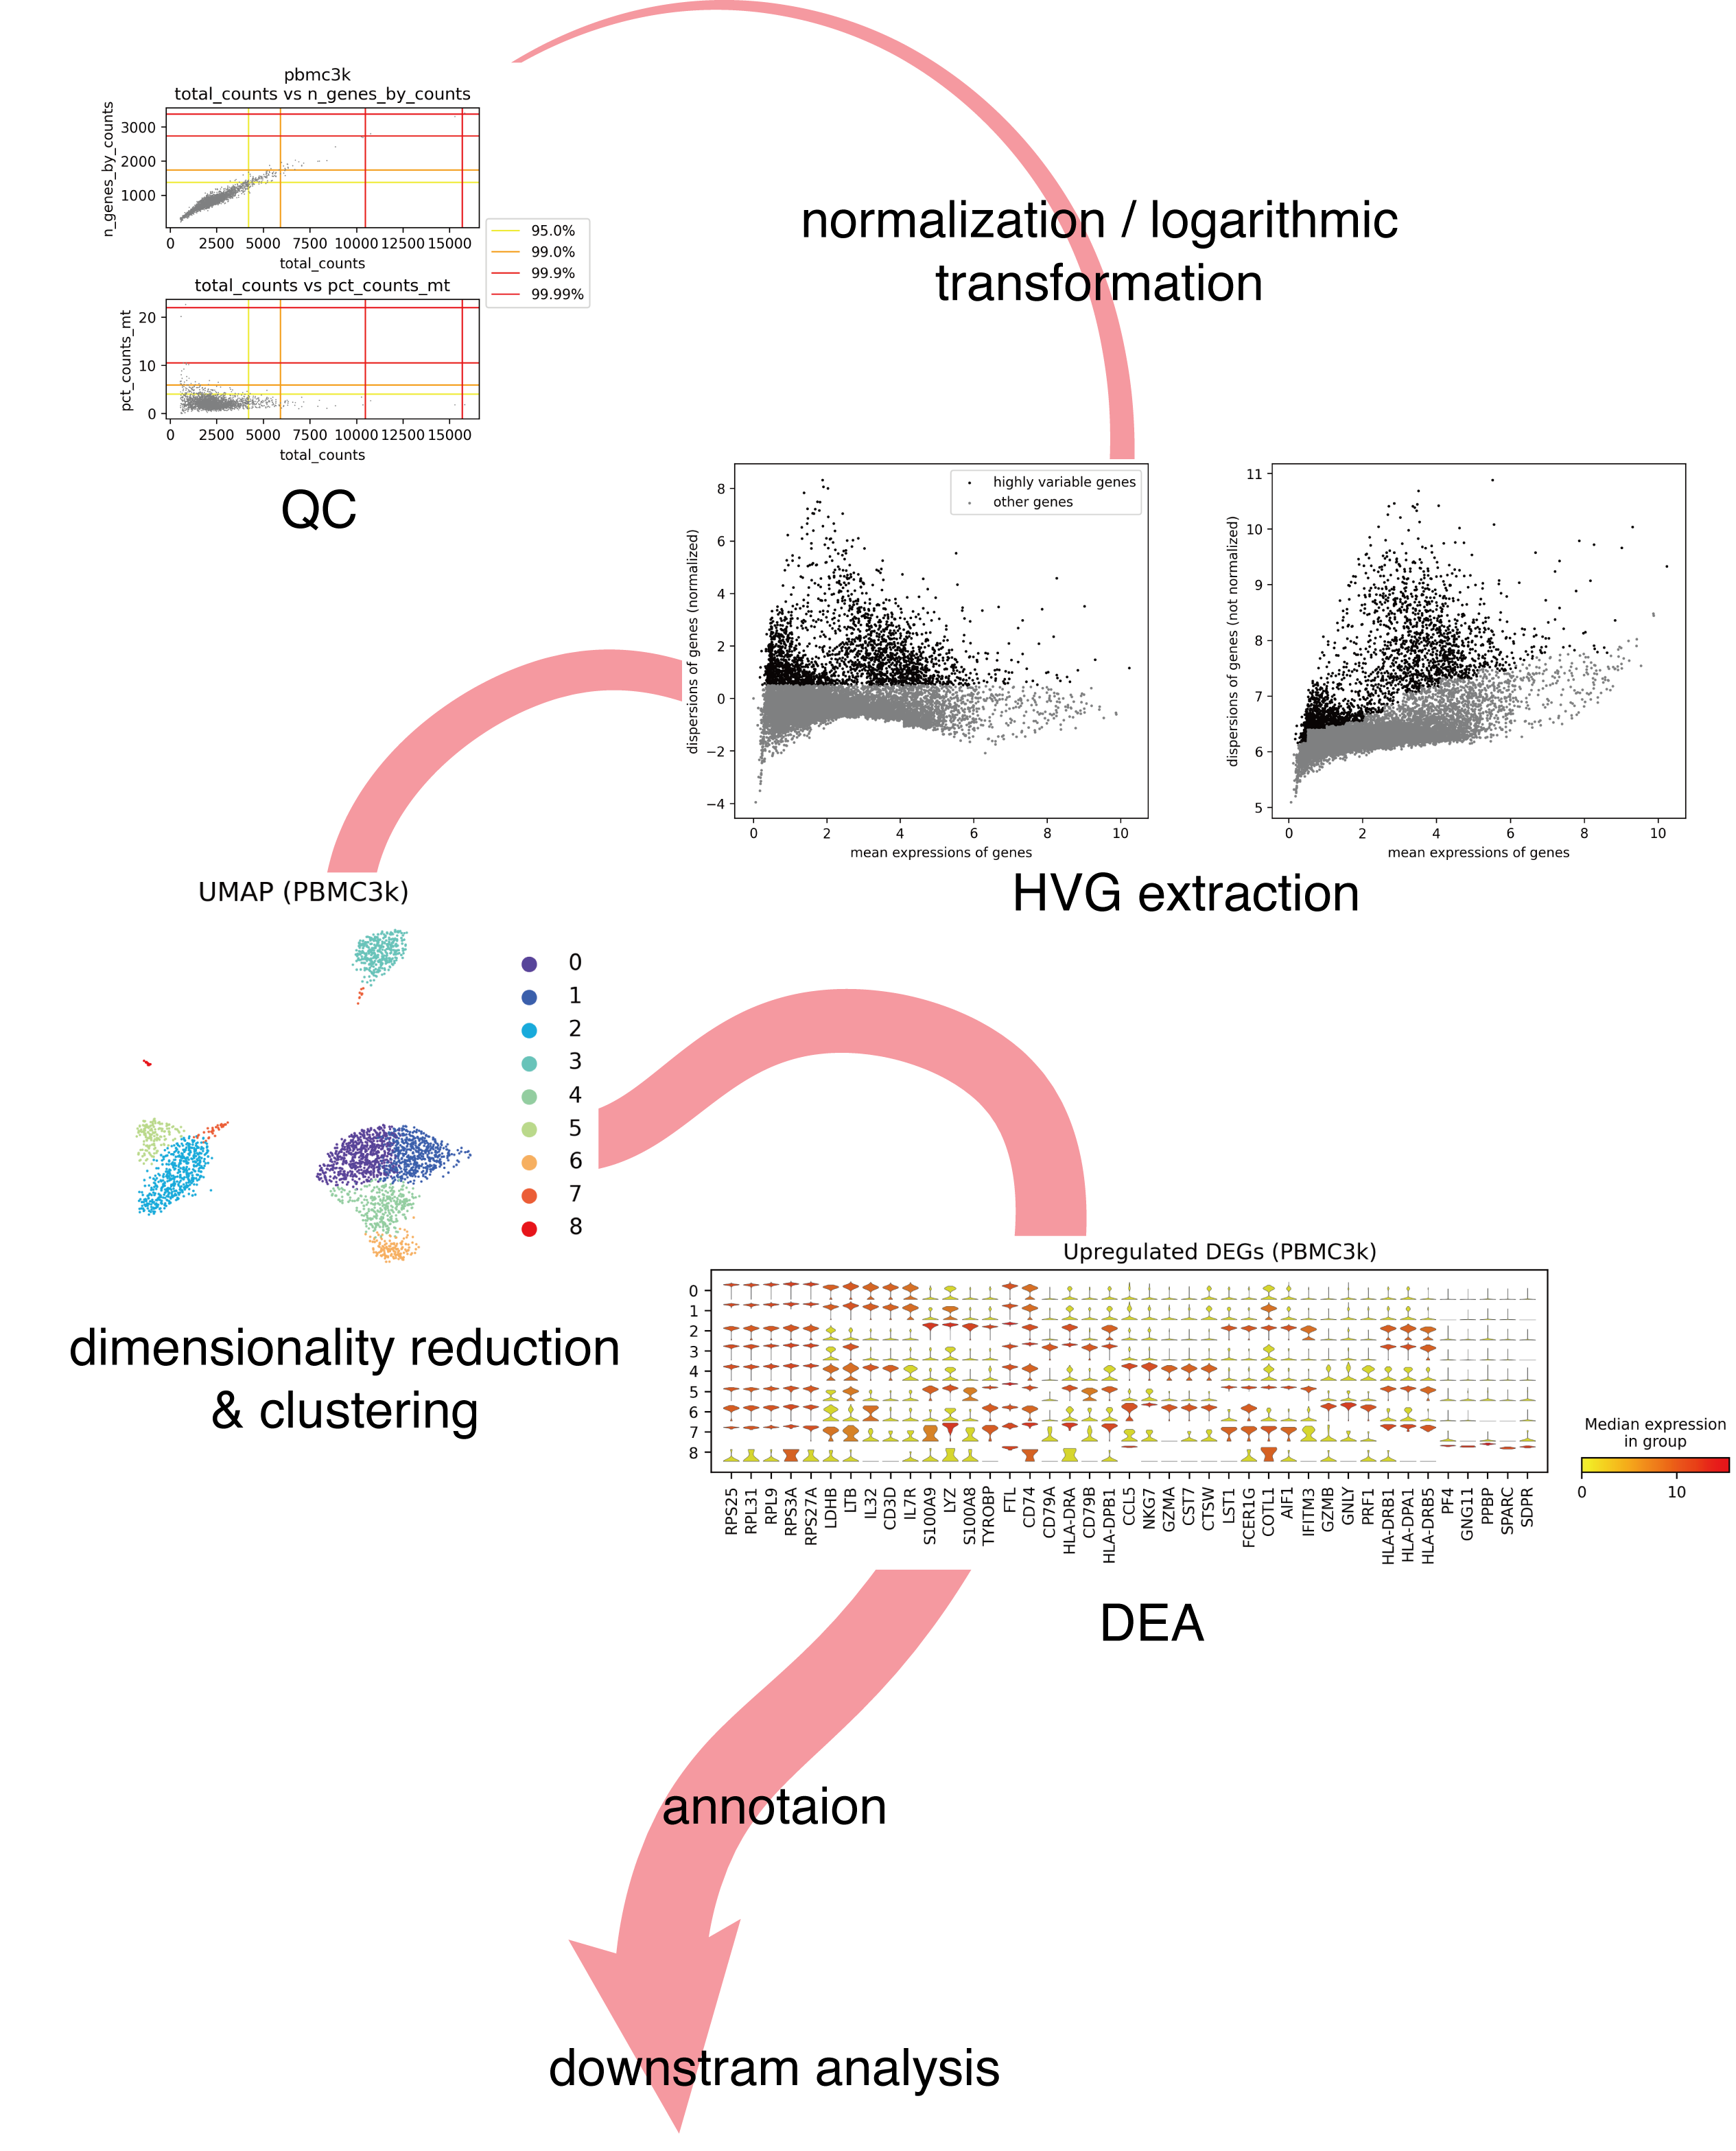
\includegraphics[scale=0.6]{./figs/exported/figure_s1.png}
  \caption{Standard workflow of scRNA-seq analysis}
  \legend{
    A scheme that shows a standard process of scRNA-seq data analysis. 
    The plots were generated during the analysis of PBMC3k.
  }
  \label{fig_s1}
\end{figure}
\begin{figure}[htb]
  \centering
  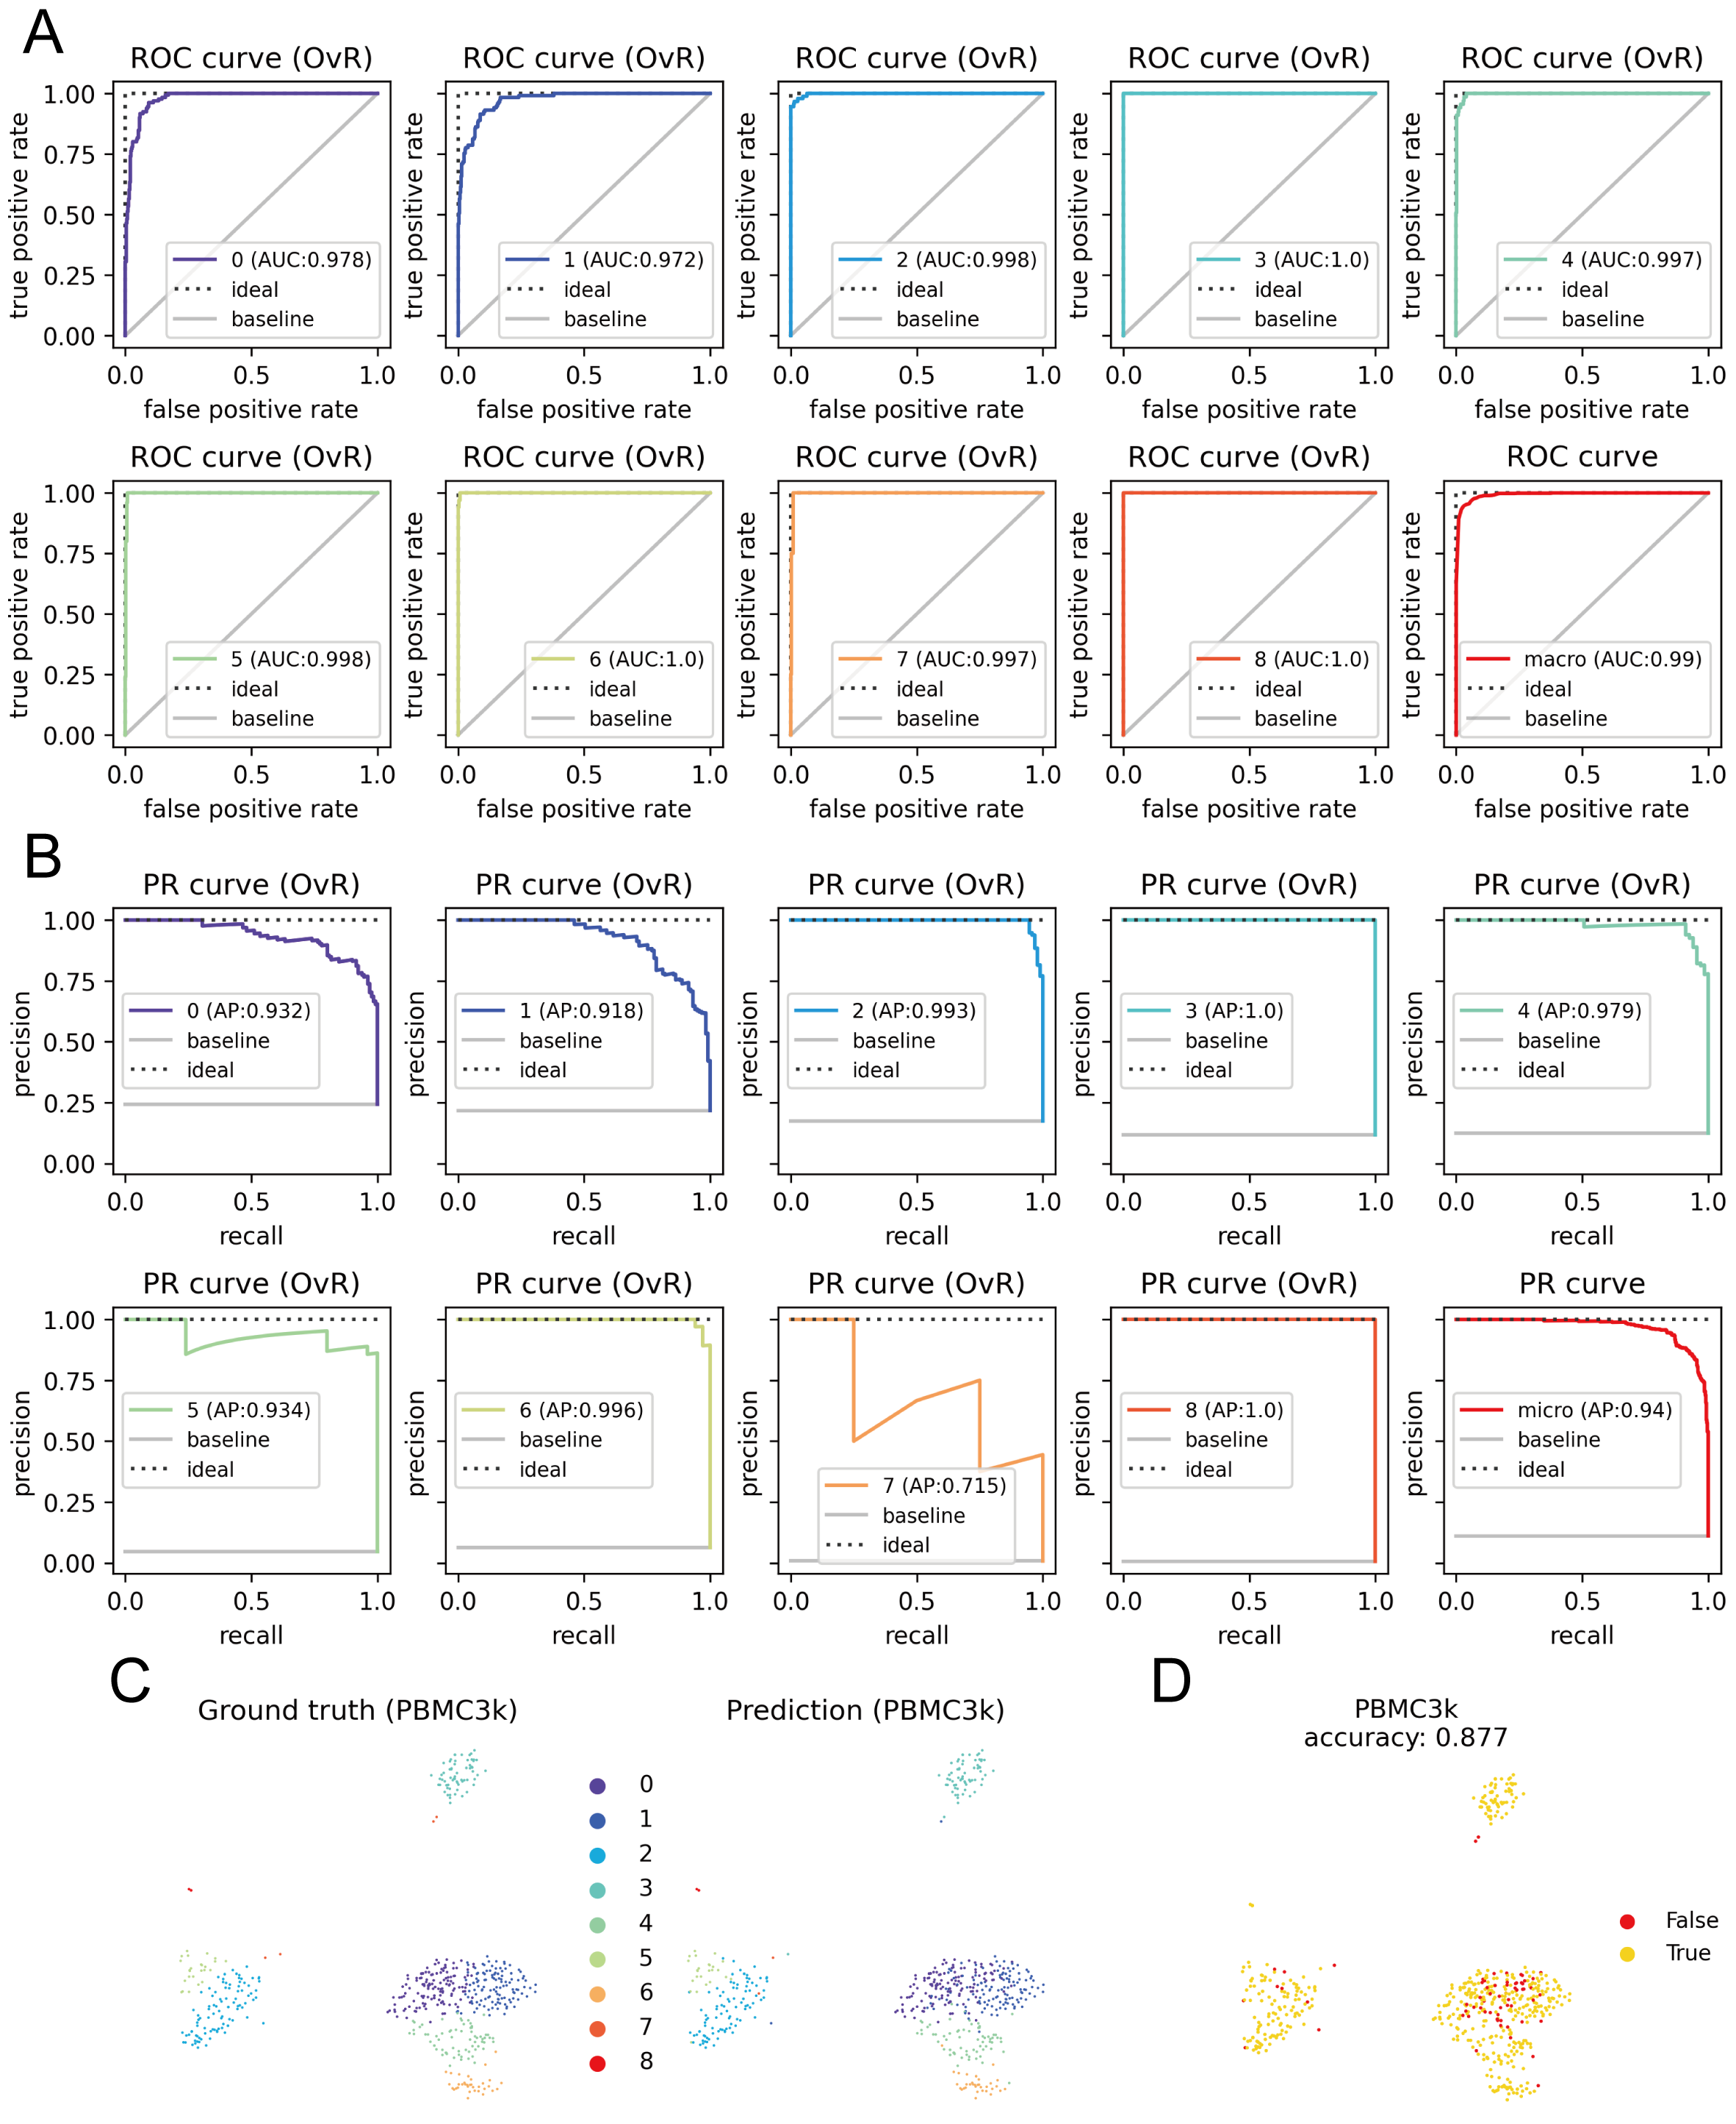
\includegraphics[scale=0.7]{./figs/exported/figure_s2.png}
  \caption{The top 5 DEGs and the GRNs of the clusters in PBMC3k}
  \legend{
    \textbf{A}: Violin plot of DEGs of the clusters (top 5 for each). 
    \textbf{B}: GRNs of the clusters. GRNs in a row share the same set of genes
    (DEGs of the subjective clusters) for the nodes
  }
  \label{fig_s2}
\end{figure}
\begin{figure}[htb]
  \centering
  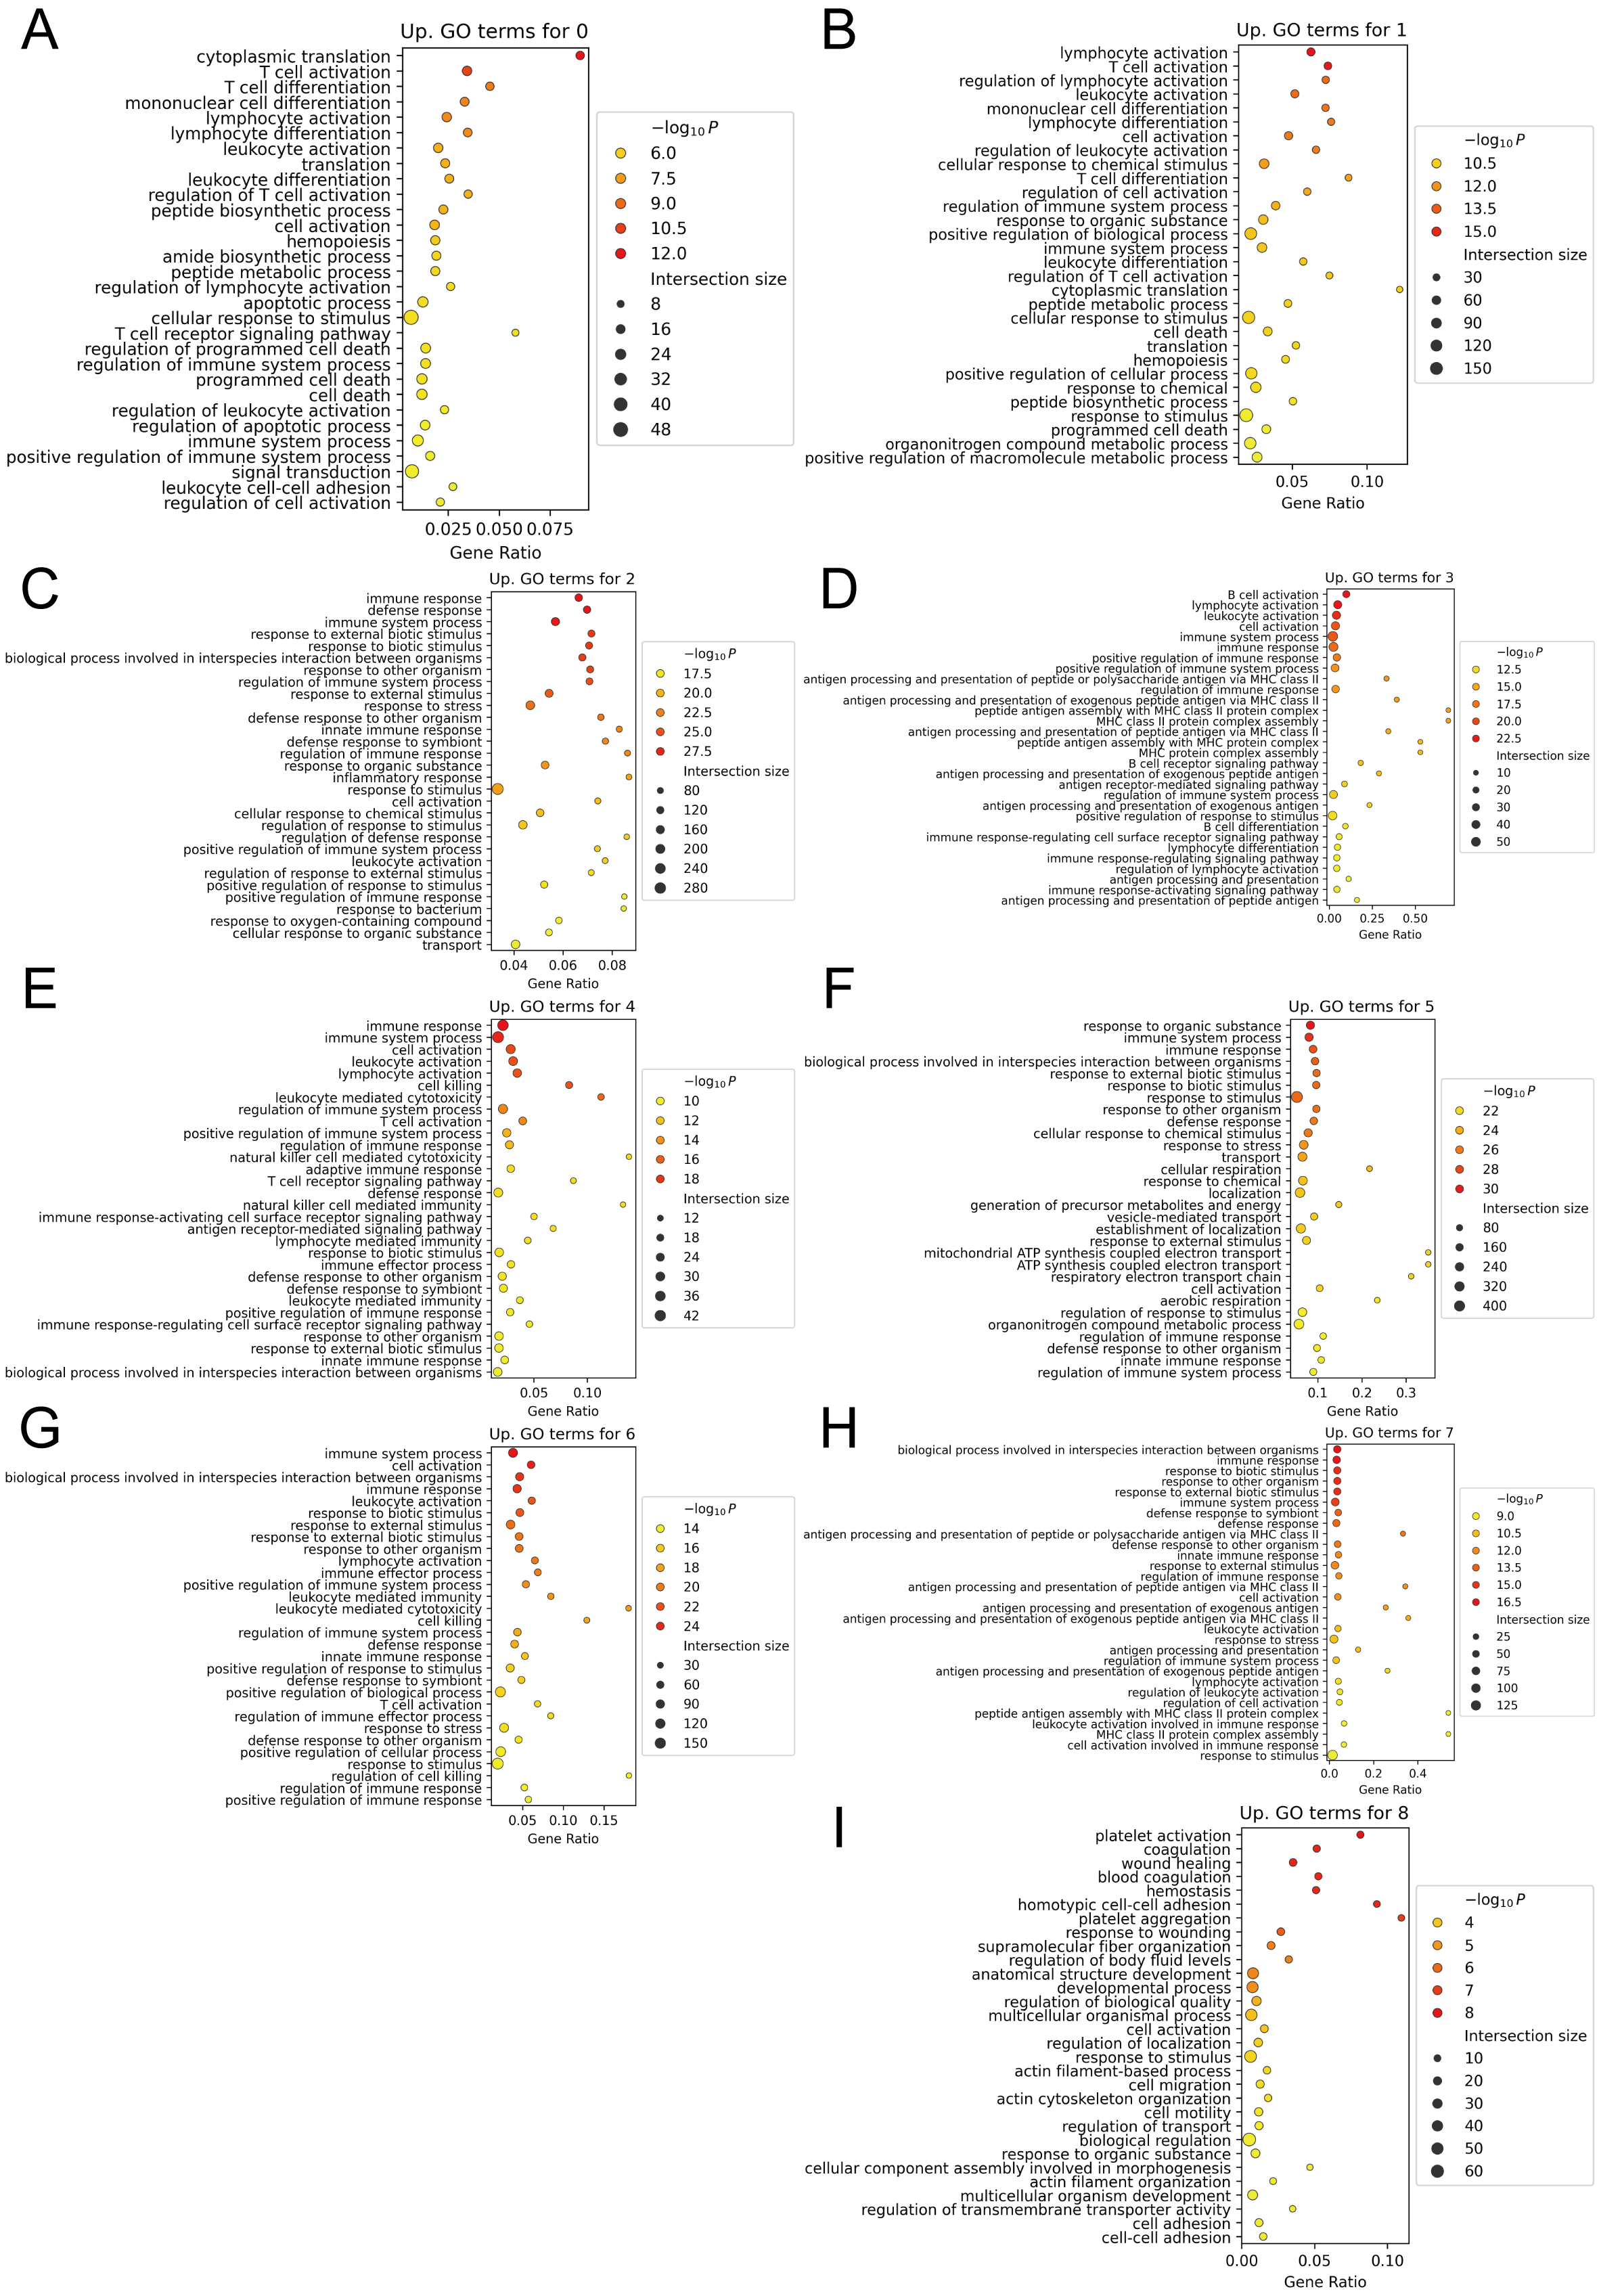
\includegraphics[scale=0.7]{./figs/exported/figure_s3.png}
  \caption{The top 10 features of the clusters in PBMC3k}
  \legend{
    \textbf{A-I}: The top 10 features (based on SHAP values) for cluster 0$\sim$8 respectively
  }
  \label{fig_s3}
\end{figure}
\begin{figure}[htb]
  \centering
  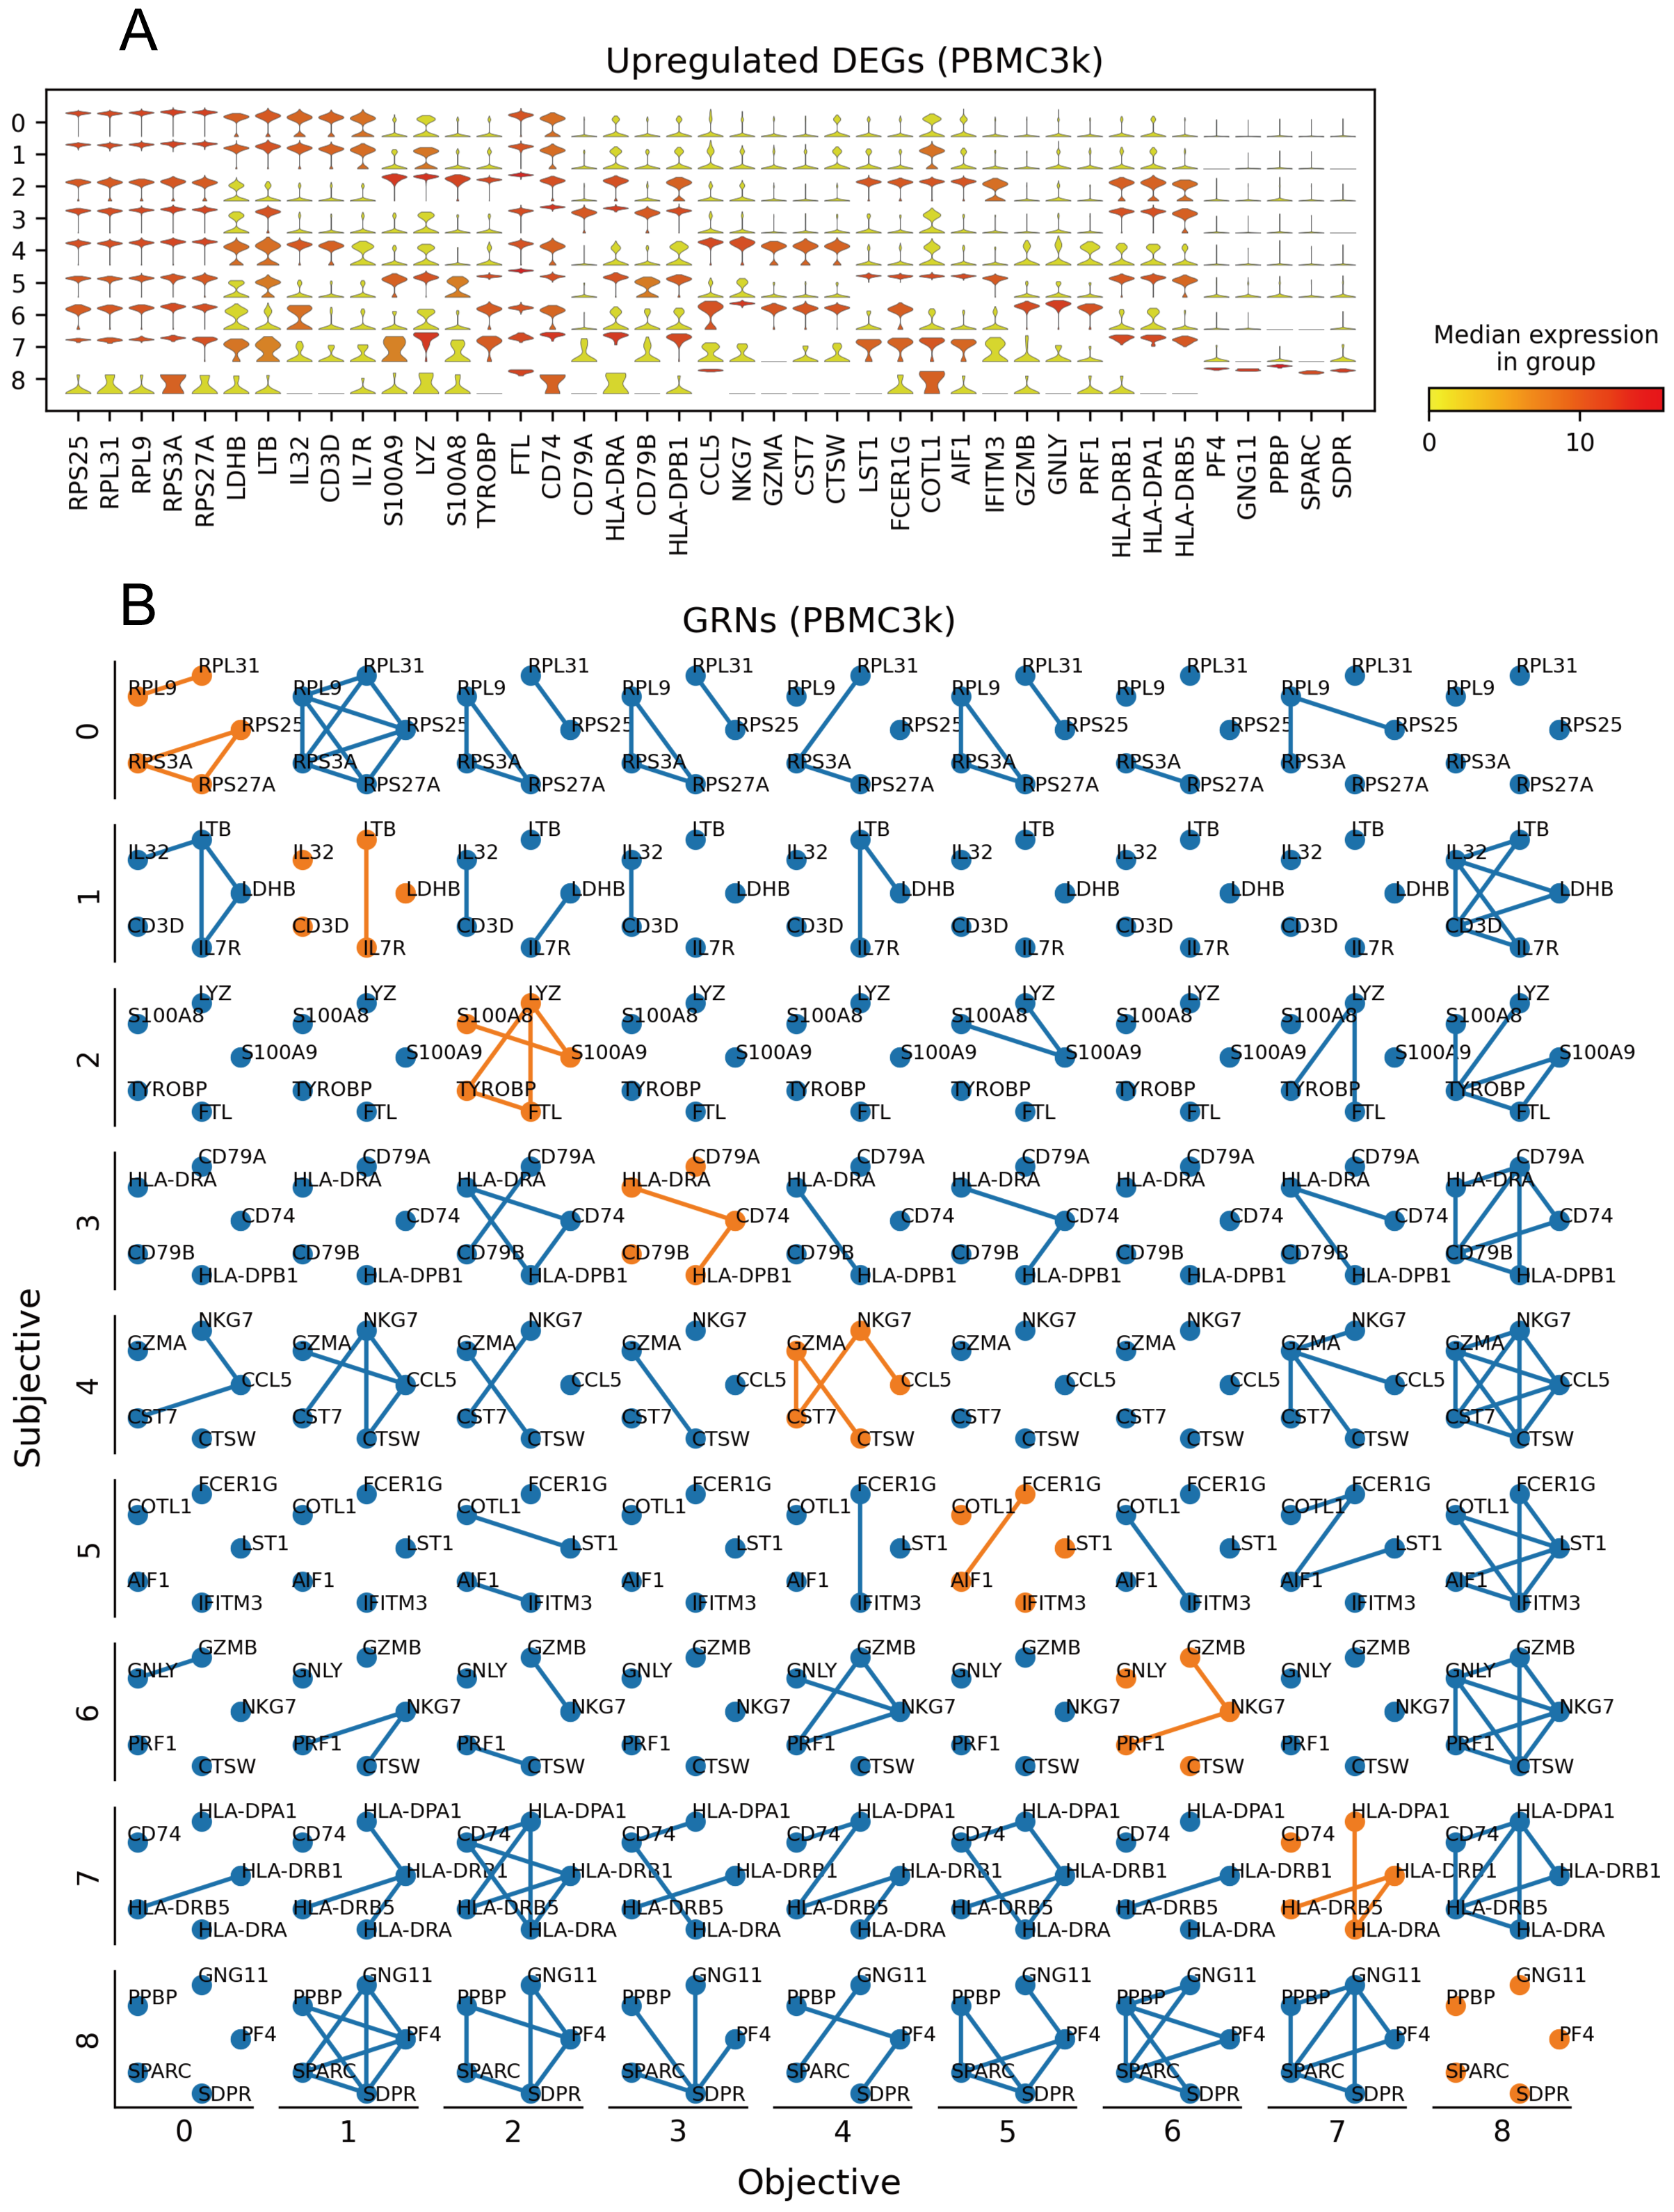
\includegraphics[scale=0.75]{./figs/exported/figure_s4.png}
  \caption{The top 5 DEGs and the GRNs of the clusters in PBMC3k}
  \legend{
    \textbf{A}: Violin plot of DEGs of the clusters (top 5 for each). 
    \textbf{B}: GRNs of the clusters. GRNs in a row share the same set of genes
    (DEGs of the subjective clusters) for the nodes
  }
  \label{fig_s4}
\end{figure}
\begin{figure}[htb]
  \centering
  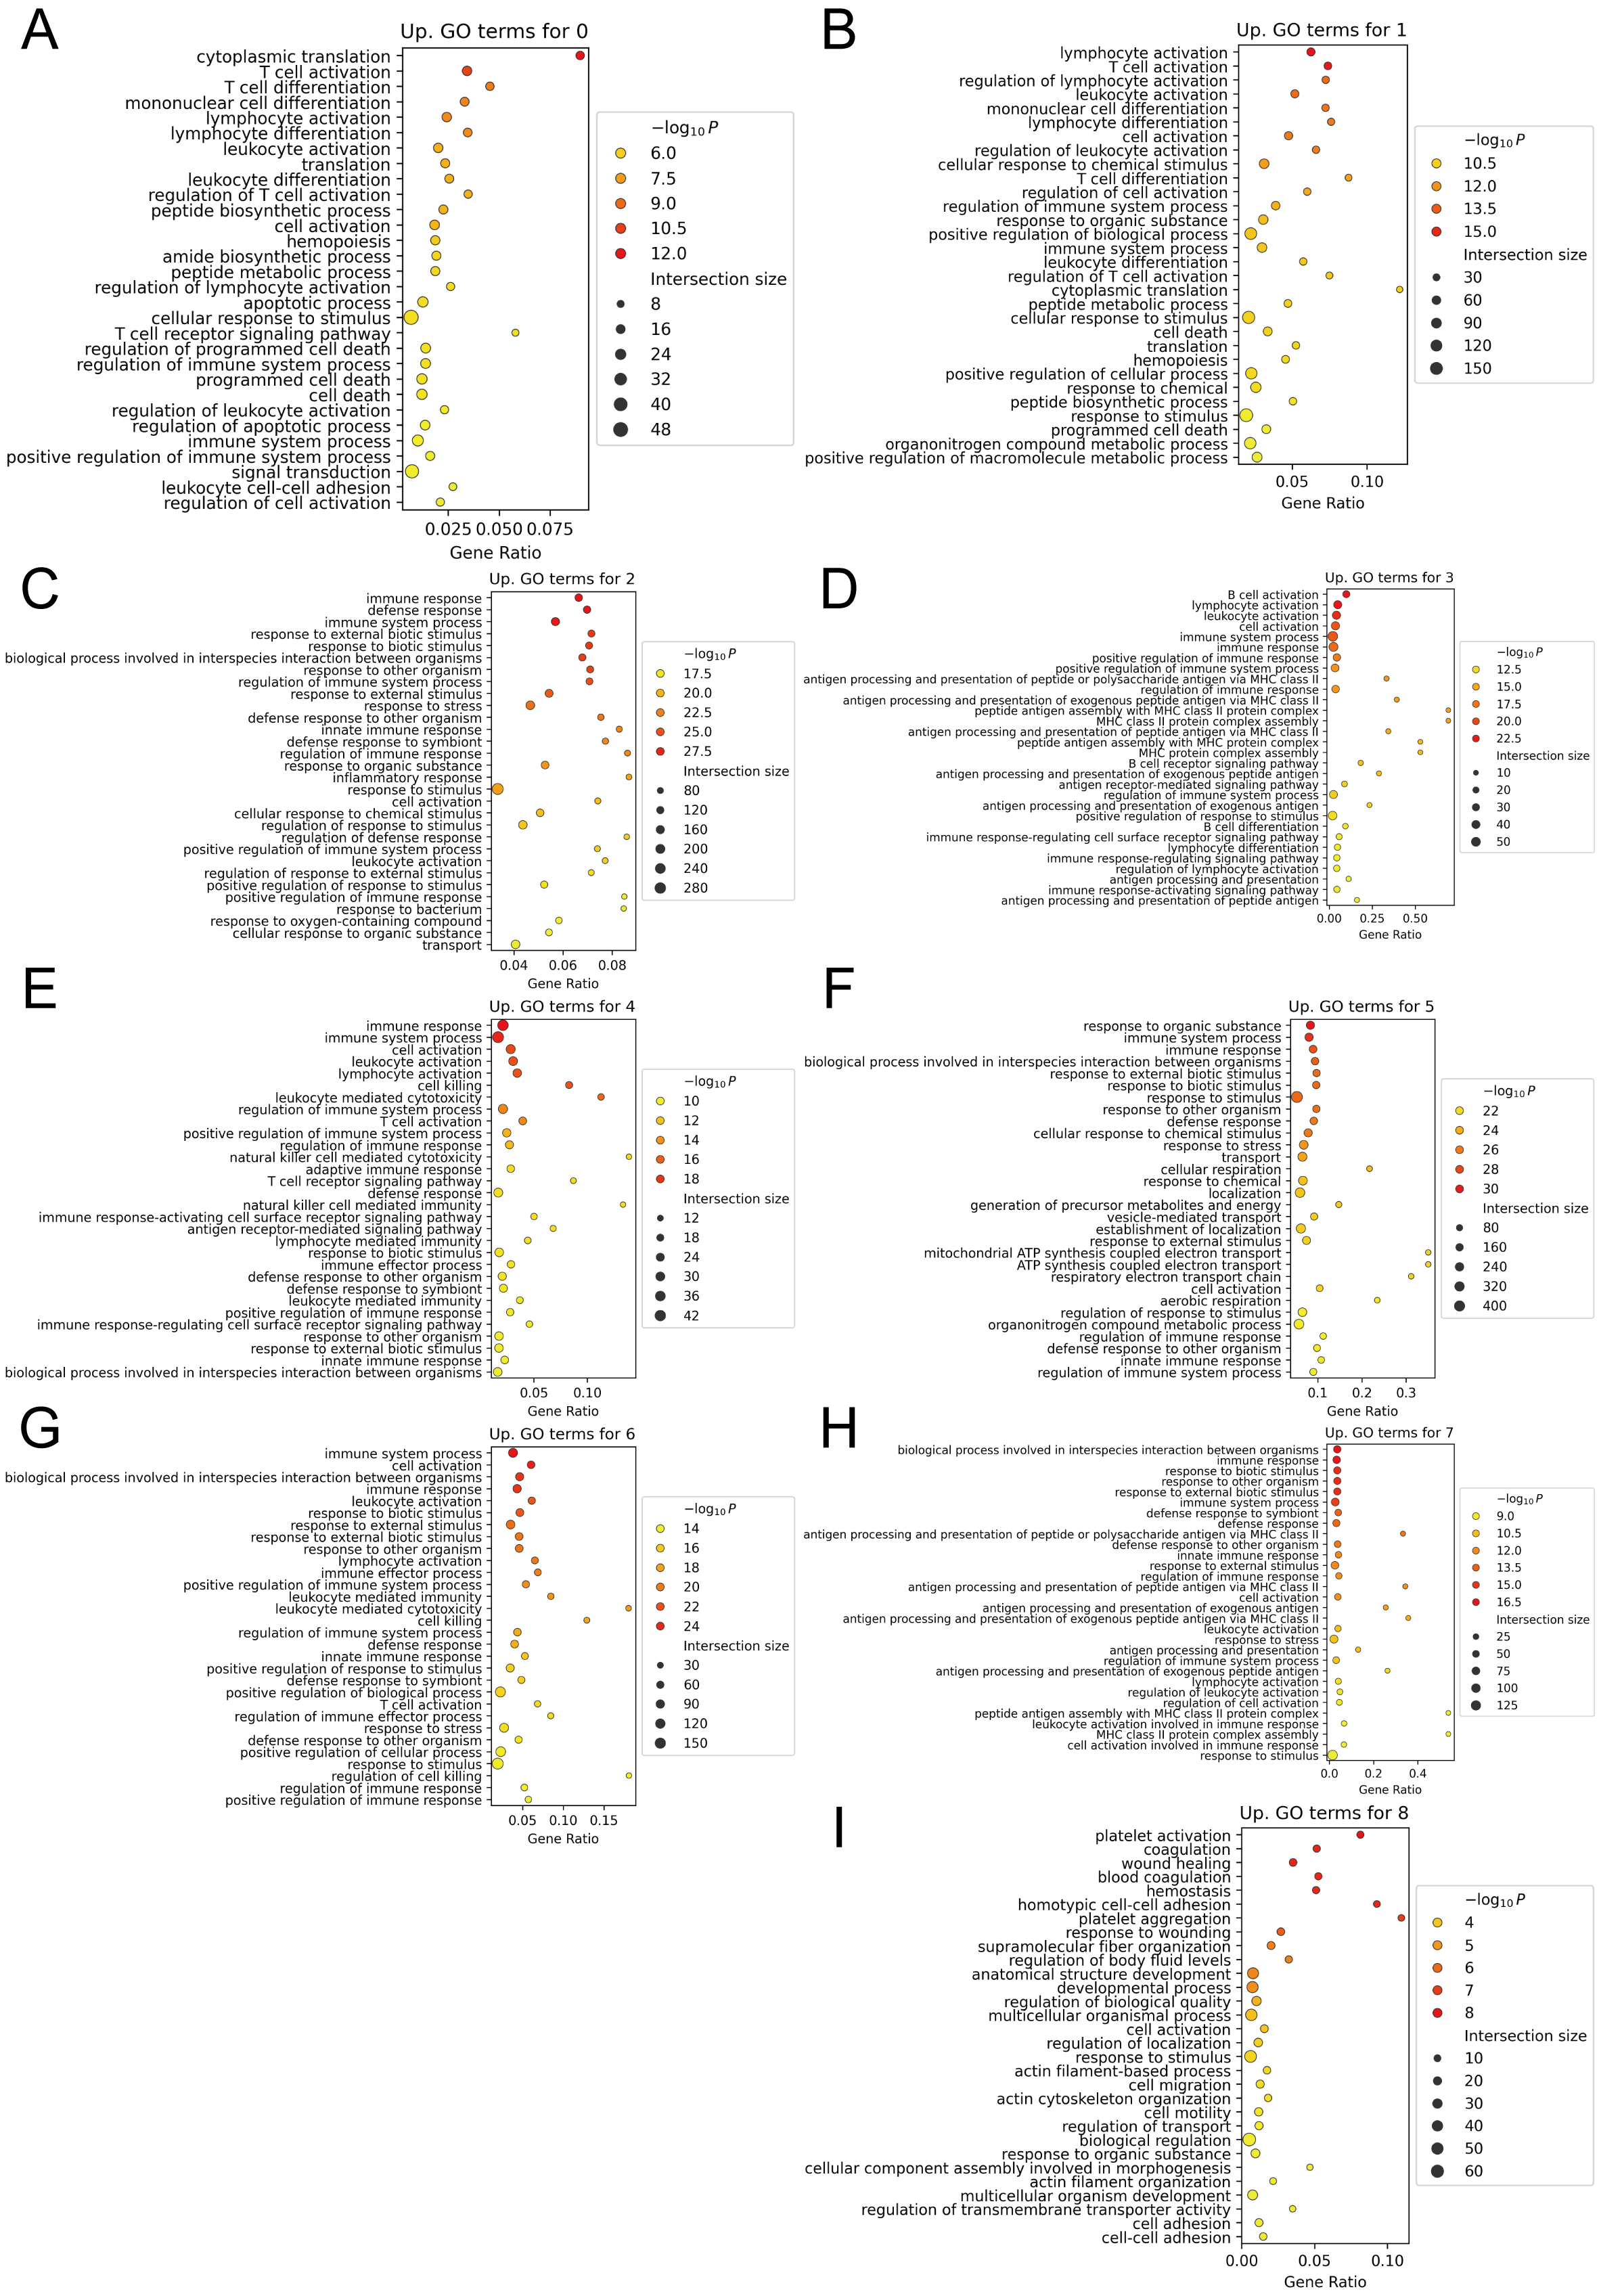
\includegraphics[scale=0.7]{./figs/exported/figure_s5.png}
  \caption{The top 30 upregulated GO terms of the clusters in PBMC3k}
  \legend{
    \textbf{A-I}: The top 30 GO terms for cluster 0$\sim$8 respectively
  }
  \label{fig_s5}
\end{figure}

\end{document}
